\documentclass[12pt]{article}

%%%%%%%%%%%%%%%%%%%%%%%%%%%%%%%%%%%%%%%%%%%%%%%%%%%%%%%%%%%%%%%%%%%%%%%%%%%%%%%%%%%%%%%%%%%%%%%%%%%%
% Math
\usepackage{fancyhdr} 
\usepackage{amsfonts}
\usepackage{amsmath}
\usepackage{amssymb}
\usepackage{amsthm}
%\usepackage{dsfont}

%%%%%%%%%%%%%%%%%%%%%%%%%%%%%%%%%%%%%%%%%%%%%%%%%%%%%%%%%%%%%%%%%%%%%%%%%%%%%%%%%%%%%%%%%%%%%%%%%%%%
% Macros
\usepackage{calc}

%%%%%%%%%%%%%%%%%%%%%%%%%%%%%%%%%%%%%%%%%%%%%%%%%%%%%%%%%%%%%%%%%%%%%%%%%%%%%%%%%%%%%%%%%%%%%%%%%%%%
% Commands and Custom Variables	
\newcommand{\problem}[1]{\hspace{-4 ex} \large \textbf{Problem #1} }
\let\oldemptyset\emptyset
\let\emptyset\varnothing
\newcommand{\norm}[1]{\left\lVert#1\right\rVert}
\newcommand{\sint}{\text{s}\kern-5pt\int}
\newcommand{\powerset}{\mathcal{P}}
\renewenvironment{proof}{\hspace{-4 ex} \emph{Proof}:}{\qed}
\newcommand{\RR}{\mathbb{R}}
\newcommand{\NN}{\mathbb{N}}
\newcommand{\QQ}{\mathbb{Q}}
\newcommand{\ZZ}{\mathbb{Z}}
\newcommand{\CC}{\mathbb{C}}
\renewcommand{\Re}{\operatorname{Re}}
\renewcommand{\Im}{\operatorname{Im}}


%%%%%%%%%%%%%%%%%%%%%%%%%%%%%%%%%%%%%%%%%%%%%%%%%%%%%%%%%%%%%%%%%%%%%%%%%%%%%%%%%%%%%%%%%%%%%%%%%%%%
%page
\usepackage[margin=1in]{geometry}
\usepackage{setspace}
%\doublespacing
\allowdisplaybreaks
\pagestyle{fancy}
\fancyhf{}
\rhead{Shaw \space \thepage}
\setlength\parindent{0pt}

%%%%%%%%%%%%%%%%%%%%%%%%%%%%%%%%%%%%%%%%%%%%%%%%%%%%%%%%%%%%%%%%%%%%%%%%%%%%%%%%%%%%%%%%%%%%%%%%%%%%
%Code
\usepackage{listings}
\usepackage{courier}
\lstset{
	language=Python,
	showstringspaces=false,
	formfeed=newpage,
	tabsize=4,
	commentstyle=\itshape,
	basicstyle=\ttfamily,
}

%%%%%%%%%%%%%%%%%%%%%%%%%%%%%%%%%%%%%%%%%%%%%%%%%%%%%%%%%%%%%%%%%%%%%%%%%%%%%%%%%%%%%%%%%%%%%%%%%%%%
%Images
\usepackage{graphicx}
\graphicspath{ {images/} }
\usepackage{float}

%tikz
\usepackage[utf8]{inputenc}
\usepackage{pgfplots}
\usepgfplotslibrary{groupplots}

%%%%%%%%%%%%%%%%%%%%%%%%%%%%%%%%%%%%%%%%%%%%%%%%%%%%%%%%%%%%%%%%%%%%%%%%%%%%%%%%%%%%%%%%%%%%%%%%%%%%
%Hyperlinks
%\usepackage{hyperref}
%\hypersetup{
%	colorlinks=true,
%	linkcolor=blue,
%	filecolor=magenta,      
%	urlcolor=cyan,
%}

\begin{document}
	\thispagestyle{empty}
	
	\begin{flushright}
		Sage Shaw \\
		m537 - Spring 2018 \\
		\today
	\end{flushright}
	
{\large \textbf{Takehome Project 1}}\bigbreak

Consider an insulated rod with end-points kept at constant temperatures $\alpha$ and $\beta$, diffusivity $D$, and internal source $q(x)$. Let $f(x)$, with $0<x<1$, be the initial distribution of the temperature in the rod. The temperature $u(x,t)$ in the rod satisfies the equations:
\begin{equation}
 \left \{
	\begin{aligned}
		\frac{\partial u}{\partial t}(x,t) & = D \frac{\partial^2u}{\partial x^2}(x,t) + q(x), && 0 <x <1, & 0&<t \\
		u(0,t) & = \alpha, \ \  u(1,t) = \beta, && & 0 & < t \\
		u(x,0) & = f(x), && 0  < x < 1
	\end{aligned} 
\right . \label{eq1}
\end{equation}
Suppose
\begin{align*}
	f(x) & = (\alpha - x)(x- \beta) \\
	 q(x) & = \pi^2\sin(\pi x) \\
	\alpha & = 1, \beta = -3, D=1
\end{align*}

\problem{1.} Determine the equilibrium solution. \bigbreak

The equilibrium solution $u_{\infty}(x)$, is the solution for which the temperature at each point is constant with respect to time. Mathematically we represent this by saying $\frac{\partial u_\infty}{\partial t} = 0$. Substituting into (\ref{eq1}) we get
\begin{align*}
0 & = D \frac{\partial^2u_\infty}{\partial x^2}(x) + q(x) \\
\frac{\partial^2u_\infty}{\partial x^2}(x) & = -\frac{1}{D}q(x) \\
& = -\pi^2 \sin(\pi x) \\
\frac{\partial u_\infty}{\partial x}(x) & = \pi \cos(\pi x) + A\\
u_\infty(x) & = \sin(\pi x) + Ax + B
\end{align*}
Using the boundary condition $u(0,t)=\alpha$ we can conclude that $B = \alpha$. Using the boundary condition $u(1,t) = \beta$ we can conclude that $A = (\beta - \alpha)$. Thus we have that 
$$
u_\infty(x) = \sin(\pi x) - 4x + 1
$$

\problem{2. } Make the substitution $v(x,t) = u(x,t) - u_\infty(x)$ and derive an initial-boundary value problem for $v(x,t)$. \bigbreak

Taking the derivative it is easy to see that $\frac{\partial v}{\partial t}(x,t) = \frac{\partial u}{\partial t}(x,t)$ since $u_\infty(x)$ is independent of $t$. Also
\begin{align*}
\frac{\partial^2v_\infty}{\partial x^2}(x,t) & = \frac{\partial^2u}{\partial x^2}(x,t) - \frac{\partial^2u_\infty}{\partial x^2}(x) \\
 & = \frac{\partial^2u}{\partial x^2}(x,t) + \pi^2\sin(\pi x) \\
 & = \frac{\partial u}{\partial t}(x,t) \\
 & = \frac{\partial v}{\partial t}(x,t)
\end{align*}

Substituting the boundary conditions we get
$$
v(0,t) = u(0,t) - u_\infty(0) = \alpha - \alpha = 0
$$
$$
v(1,t) = u(1,t) - u_\infty(1) = \beta - \big( (\beta - \alpha)1 + \alpha \big) = 0
$$
Substituting our initial condition we get
$$
v(x,0) = u(x,0) - u_\infty(x) = (1 - x)(x + 3) - \sin(\pi x) + 4x - 1
$$
Collecting these, we have created a homogeneous initial-boundary value problem:
\begin{equation}
\left \{
	\begin{aligned}
		\frac{\partial v}{\partial t}(x,t) & = \frac{\partial^2v}{\partial x^2}(x,t), && 0 <x <1, & 0&<t \\
		v(0,t) & = 0, \ \  v(1,t) = 0, && & 0 & < t \\
		v(x,0) & = (1 - x)(x + 3) - \sin(\pi x) + 4x - 1, && 0  < x < 1
	\end{aligned} 
\right . \label{eq2}
\end{equation}

\problem{3. } From our notes we know that a solution to (\ref{eq2}) is given by
$$
v(x,t) = \sum\limits_{n=1}^\infty b_n \sin(\frac{n \pi}{L}x)e^{-k (\frac{n \pi}{L})^2t}
$$
where the coefficients $b_n$ are given by
$$
b_n = \frac{2}{L}\int_{0}^{L}f(x) \sin(\frac{n \pi}{L}x) dx
$$
Here $L = 1$, and 
\begin{align*}
f(x) & = (1 - x)(x + 3) - \sin(\pi x) + 4x - 1 \\
& = -x^2 - 2x + 3 - \sin(\pi x) + 4x - 1 \\
& = -x^2 + 2x + 2 - \sin(\pi x)
\end{align*}
We can calculate $b_n$ for $n \in \{1, 2, ...\}$ as follows
\begin{align*}
	b_n & = 2\int_{0}^{1}f(x) \sin(n \pi x) dx \\
	& = -2\int_{0}^{1}x^2 \sin(n \pi x) dx + 4 \int_{0}^{1}x \sin(n \pi x) dx \\
	& \phantom{===} + 4 \int_{0}^{1} \sin(n \pi x) dx - 2\int_{0}^{1} \sin(\pi x)\sin(n \pi x) dx
\end{align*}
We will consider all four of these integrals separately. First
\begin{align*}
	\int_{0}^{1}x^2 \sin(n \pi x) dx & = \int_{0}^{1}x^2 \bigg[ \frac{-1}{n \pi}\cos(n \pi x) \bigg]^{\prime} dx \\
	& = \bigg[ x^2 \frac{-1}{n \pi}\cos(n \pi x) \bigg]_{x=0}^{x=1}  + \frac{2}{n \pi} \int_{0}^{1} x \cos(n \pi x) dx \\
	& = \frac{-1}{n \pi}\cos(n \pi) + \frac{2}{n \pi} \int_{0}^{1} x \bigg[\frac{1}{n \pi}\sin(n \pi x) \bigg]^{\prime} dx \\
	& = \frac{(-1)^{n+1}}{n \pi} + \frac{2}{n \pi} \int_{0}^{1} x \bigg[\frac{1}{n \pi}\sin(n \pi x) \bigg]^{\prime} dx \\
	& = \frac{(-1)^{n+1}}{n \pi} + \bigg[ \frac{2}{n \pi} x\frac{1}{n \pi}\sin(n \pi x) \bigg]_{x=0}^{x=1} - \frac{2}{n \pi}\int_{0}^{1} \frac{1}{n \pi}\sin(n \pi x) dx \\
	& = \frac{(-1)^{n+1}}{n \pi} - \frac{2}{n^2 \pi^2}\int_{0}^{1} \sin(n \pi x) dx \\
	& = \frac{(-1)^{n+1}}{n \pi} + \frac{2}{n^3 \pi^3} \bigg[ \cos(n \pi x) \bigg]_{x=0}^{x=1} \\
	& = \frac{(-1)^{n+1}}{n \pi} + \frac{2}{n^3 \pi^3} \bigg[ \cos(n \pi)  - 1\bigg] \\
	& = \frac{(-1)^{n+1}}{n \pi} + \frac{2(-1)^{n}}{n^3 \pi^3} - \frac{2}{n^3 \pi^3} \\
\end{align*}
Next
\begin{align*}
	\int_{0}^{1}x \sin(n \pi x) dx & = \int_{0}^{1}x \bigg[ \frac{-1}{n \pi}\cos(n \pi x) \bigg]^{\prime}dx \\
	&= \bigg[ -x \frac{1}{n \pi}\cos(n \pi x) \bigg]_{x=0}^{x=1} + \frac{1}{n \pi} \int_{0}^{1} \cos(n \pi x) dx \\
	& = \frac{-1}{n \pi}\cos(n \pi) + \frac{1}{n \pi} \bigg[ \frac{1}{n \pi} \sin(n \pi x) \bigg]_{x=0}^{x=1} \\
	& = \frac{(-1)^{n+1}}{n\pi}
\end{align*}
Next
\begin{align*}
	\int_{0}^{1}\sin(n \pi x) dx & = \bigg[ \frac{-1}{n\pi} \cos(n \pi x) \bigg]_{x=0}^{x=1} \\
	& = \frac{-1}{n\pi} \cos(n \pi) - \frac{-1}{n\pi} \\
	& = \frac{(-1)^{n+1}}{n\pi} + \frac{1}{n\pi} \\
	& = \frac{1 + (-1)^{n+1}}{n\pi}
\end{align*}
Lastly from our orthogonality rules we know that 
$$
\int_0^1 sin(n \pi x) sin(\pi x) dx = \begin{cases}
	\frac{1}{2} & \text{ if } n=1 \\
	0 & \text{else}
\end{cases}
$$

From these four results it is appropriate to consider 4 cases: when $n=1$, when $n$ is even, and when $n$ is odd and greater than 1. When $n = 1$ we have
\begin{align*}
	b_n & = -2\int_{0}^{1}x^2 \sin(n \pi x) dx + 4 \int_{0}^{1}x \sin(n \pi x) dx \\
	& \phantom{===} + 4 \int_{0}^{1} \sin(n \pi x) dx - 2\int_{0}^{1} \sin(\pi x)\sin(n \pi x) dx \\
	b_1 & = -2 \bigg( \frac{1}{\pi} - \frac{2}{\pi^3} - \frac{2}{\pi^3}\bigg) + 4 \bigg( \frac{1}{\pi} \bigg) + 4 \bigg( \frac{2}{\pi} \bigg) - 2 \bigg( \frac{1}{2} \bigg) \\
	& = \frac{10}{\pi} + \frac{8}{\pi^3} - 1 \\
	& \approx 2.441111137303503
\end{align*}
When $n$ is even we have
\begin{align*}
b_n & = -2\int_{0}^{1}x^2 \sin(n \pi x) dx + 4 \int_{0}^{1}x \sin(n \pi x) dx \\
& \phantom{===} + 4 \int_{0}^{1} \sin(n \pi x) dx - 2\int_{0}^{1} \sin(\pi x)\sin(n \pi x) dx \\
b_n & = -2 \bigg( \frac{-1}{n\pi} + \frac{2}{n^3\pi^3} - \frac{2}{n^3\pi^3}\bigg) + 4 \bigg( \frac{-1}{n\pi} \bigg) + 4 \bigg( 0 \bigg) - 2 \bigg( 0 \bigg) \\
& = \frac{-2}{n\pi}
\end{align*}
Lastly when $n$ is odd and $1<n$ we have
\begin{align*}
b_n & = -2\int_{0}^{1}x^2 \sin(n \pi x) dx + 4 \int_{0}^{1}x \sin(n \pi x) dx \\
& \phantom{===} + 4 \int_{0}^{1} \sin(n \pi x) dx - 2\int_{0}^{1} \sin(\pi x)\sin(n \pi x) dx \\
b_n & = -2 \bigg( \frac{1}{n\pi} + \frac{-2}{n^3\pi^3} - \frac{2}{n^3\pi^3}\bigg) + 4 \bigg( \frac{1}{n\pi} \bigg) + 4 \bigg( \frac{2}{n\pi} \bigg) - 2 \bigg( 0 \bigg) \\
& = \frac{10}{n\pi} + \frac{8}{n^3 \pi^3}
\end{align*}

Combining all of these facts we get that 
\begin{align*}
	u(x,t) & = \sin(\pi x) - 4x + 1 + \sum\limits_{n=1}^\infty b_n \sin(n \pi x)e^{-(n \pi)^2t} \\
	b_n & = \begin{cases}
			\frac{10}{\pi} + \frac{8}{\pi^3} - 1 &, n=1 \\
			\frac{-2}{n\pi} & , n \text{ even} \\
			\frac{10}{n\pi} + \frac{8}{n^3 \pi^3} & \text{, else}
		\end{cases}
\end{align*}
for $0<x<1$ and $t>0$ is the full solution to (\ref{eq1}).

\problem{4. } The solution for this problem can be visualized via the following contour plot.

\begin{figure}[H]
	\caption{Contour Plot of $u(x,t)$ with $n=10$ terms of the series.}
	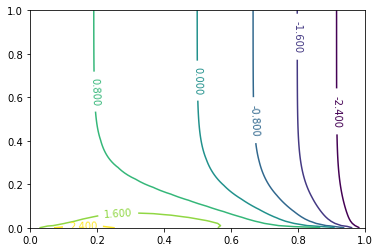
\includegraphics[width=.9\textwidth]{tk01_figure_1_contour_10}
	\label{contour10}
	\centering
\end{figure}
\begin{figure}[H]
	\caption{Contour Plot of $u(x,t)$ with $n=10$ terms of the series.}
	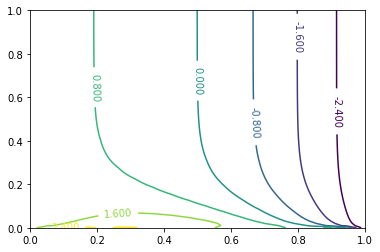
\includegraphics[width=.9\textwidth]{tk01_figure_2_contour_200}
	\label{contour200}
	\centering
\end{figure}

Very few terms of the series need to be computed to have a highly accurate approximation of the function. It seems that somewhere between 2 and 5 is the cutoff point, but just to demonstrate, we can see that there is no visible difference between $n=10$ terms and $n=200$ terms. \bigbreak

For very small $t$ values, there is more error due to the fact that the coefficients $b_n$ oscillate and converge very slowly. This is fixed very quickly since the term $e^{-(n \pi)^2t}$ converges rapidly to zero. To demonstrate this, consider a cross-section when $t=0.0005$ for different numbers of terms in the series.
	
	
\begin{figure}[H]
	\caption{$u_\infty(x,.0005)$}
	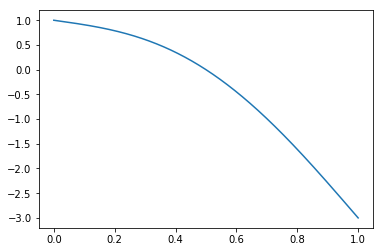
\includegraphics[width=.5\textwidth]{tk01_figure_3_cross0}
	\label{cross0}
	\centering
\end{figure}
\begin{figure}[H]
	\caption{$u(x,.0005)$ approximated with $n=1$ terms}
	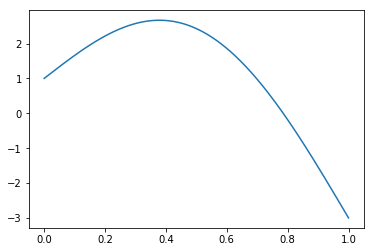
\includegraphics[width=.5\textwidth]{tk01_figure_4_cross1}
	\label{fig2}
	\centering
\end{figure}
\begin{figure}[H]
	\caption{$u(x,.0005)$ approximated with $n=2$ terms}
	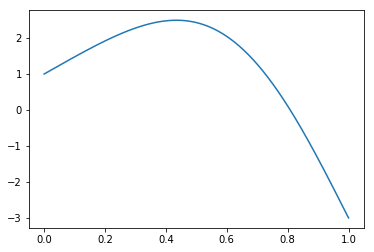
\includegraphics[width=.5\textwidth]{tk01_figure_5_cross2}
	\label{fig2}
	\centering
\end{figure}
\begin{figure}[H]
	\caption{$u(x,.0005)$ approximated with $n=5$ terms}
	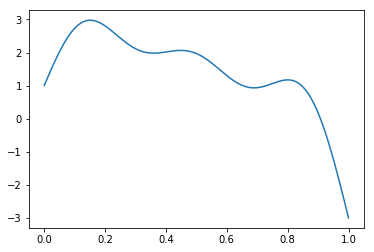
\includegraphics[width=.5\textwidth]{tk01_figure_6_cross5}
	\label{fig2}
	\centering
\end{figure}
\begin{figure}[H]
	\caption{$u(x,.0005)$ approximated with $n=10$ terms}
	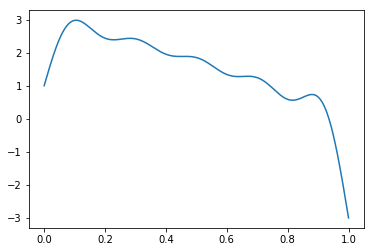
\includegraphics[width=.5\textwidth]{tk01_figure_7_cross10}
	\label{fig2}
	\centering
\end{figure}
\begin{figure}[H]
	\caption{$u(x,.0005)$ approximated with $n=1000$ terms}
	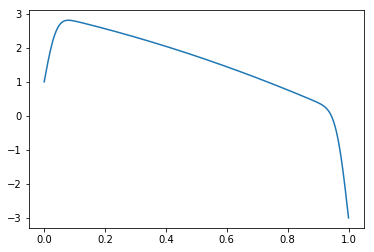
\includegraphics[width=.5\textwidth]{tk01_figure_8_cross1000}
	\label{fig2}
	\centering
\end{figure}

In conclusion, if $t$ is not very small only a few iterations are needed - certainly $10$ is enough. For very small values of $t \approx 0$, the exponential terms is roughly $e^{-(n \pi)^2t} \approx 1$ and thus it converges at approximately the same rate as $b_n$ converges which has the same order of convergence as the alternating harmonic series, which is known to be extremely slow.

\end{document}
